\documentclass[11pt,a4paper]{report} 

% Für doppelseitigen Ausdruck (nur bei > 60 Seiten sinnvoll)
% \usepackage{ifthen}
% \usepackage[german]{babel}
% \setboolean{@twoside}{true}
% \setboolean{@openright}{true}

% Deutsch
\usepackage[german]{babel} % deutsch und deutsche Rechtschreibung
\usepackage[utf8]{inputenc} % Unicode Text 
\usepackage[T1]{fontenc} % Umlaute und deutsches Trennen
\usepackage{textcomp} % Euro
\usepackage[hyphens]{url}
% statt immer Ab\-schluss\-ar\-beit zu schreiben
% einfach hier sammeln mit -. 
\hyphenation{Ab-schluss-ar-beit}
% Vorsicht bei Umlauten und Bindestrichen
\hyphenation{Ver-st\"ar-ker-aus-gang}
 % eigene Hyphenations, die für das Dokument gelten
\usepackage{amssymb} % Symbole
\usepackage{emptypage} % Wirklich leer bei leeren Seiten
\usepackage[table]{xcolor}

%% Fonts, ein kompletter Satz an Optionen
% Times New Roman, gewohnter Font, ok tt und serifenlos
%\usepackage{mathptmx} 
%\usepackage[scaled=.95]{helvet}
%\usepackage{courier}

% Palatino mit guten Fonts für tt und serifenlos
\usepackage{mathpazo} % Palatino, mal was anderes
\usepackage[scaled=.95]{helvet}
\usepackage{courier}

% New Century Schoolbook sieht auch nett aus (macht auch tt und serifenlos)
%\usepackage{newcent}

% Oder default serifenlos mit Helvetica 
% ich kann es nicht mehr sehen ...
%\renewcommand{\familydefault}{\sfdefault}

\usepackage{microtype}

% Bilder und Listings
\usepackage{graphicx} % wir wollen Bilder einfügen
\usepackage{subfig} % Teilbilder
\usepackage{wrapfig} % vielleicht doch besser vermeiden
\usepackage{listings} % schöne Quellcode-Listings
% ein paar Einstellungen für akzeptable Listings
\lstset{basicstyle=\ttfamily, columns=[l]flexible, mathescape=true, showstringspaces=false, numbers=left, numberstyle=\tiny}
\lstset{language=python} % und nur schöne Programmiersprachen ;-)
% und eine eigene Umgebung für Listings
\usepackage{float}
\newfloat{listing}{htbp}{scl}[chapter]
\floatname{listing}{Listing}

% URL-Weiterleitungen
\usepackage{hyperref}

% Kommentare im Code optimieren
\usepackage{verbatim}

% Seitenlayout
\usepackage[paper=a4paper,width=16.3cm,left=20mm,height=23.5cm]{geometry}
\usepackage{setspace}
\linespread{1.15}
\setlength{\parskip}{0.5em}
\setlength{\parindent}{0em} % im Deutschen Einrückung nicht üblich, leider

% Seitenmarkierungen 
\newcommand{\phv}{\fontfamily{phv}\fontseries{m}\fontsize{9}{11}\selectfont}
\usepackage{fancyhdr} % Schickere Header und Footer
\pagestyle{fancy}
\renewcommand{\chaptermark}[1]{\markboth{#1}{}}
%\fancyhead[L]{\phv \leftmark}
\fancyhead[RE,LO]{\phv \nouppercase{\leftmark}}
\fancyhead[LE,RO]{\phv \thepage}
% Unten besser auf alles Verzichten
%\fancyfoot[L]{\textsf{\small \kurztitel}}
\fancyfoot[C]{\ } % keine Seitenzahl unten

% Theorem-Umgebungen
\newtheorem{definition}{Definition}[chapter]
\newtheorem{satz}{Satz}[chapter]
\newtheorem{lemma}[satz]{Lemma} % gleicher Zähler wie Satz
\newtheorem{theorem}{Theorem}[chapter]
\newenvironment{beweis}[1][Beweis]{\begin{trivlist}
\item[\hskip \labelsep {\textit{#1 }}]}{\end{trivlist}}
\newcommand{\qed}{\hfill \ensuremath{\square}}

% Quellen teilen
\usepackage{bibtopic} 

% Hochschule Logo, noch nicht perfekt
\usepackage{hsrmlogo}

% Spezialpakete
\usepackage{epigraph}
\setlength{\epigraphrule}{0pt} % kein Trennstrich

% damit wir nicht so viel tippen müssen, nur für Demo 
\usepackage{blindtext} 

% Zum Zeigen von Fehlern
\usepackage{soul}
\newcommand*\falsch{\st}

% Kapitelüberschriften ohne Zahl und Überschrift
\makeatletter
\def\@makechapterhead#1{%
  \vspace*{0\p@}%
  {\parindent \z@ \raggedright \normalfont
    \interlinepenalty\@M
    % \Huge\bfseries \thechapter.\quad #1\par\nobreak
    \Huge\bfseries #1\par
    \vskip 20\p@
  }}
\makeatother
 % alle Pakete und Einstellungen

% Hier anpassen 
\newcommand{\kurztitel}{Anlagen}
\newcommand{\titel}{Businessplan zur Etablierung von ARTIFY}
\newcommand{\fach}{Seminar: Entrepreneurship RheinMain } % Hier Fach nennen 
\newcommand{\autor}{Jonas Rittirsch}
\newcommand{\ort}{Wiesbaden}

\begin{document}
\begin{titlepage}
  \begin{center}
    % Kopf der Seite
    \hsrmlogo[1]
    \parbox[t]{8cm}{
      % \textsf würde das Aussehen der ersten Seite ruinieren, 
      % wer will, soll das selbst außen rum machen...
      \textbf{Hochschule RheinMain}\\
      Fachbereich DCSM\\
      Studiengang Wirtschaftsinformatik}
    \vfill    
    {\LARGE Seminar- und Studienleistung} \\[0.5cm]
    {\large als Ergänung des zu bewertenden Pitches} \\[5mm]
    {\large \textbf{\fach} } \\[5mm]
    \rule{\textwidth}{1pt}\\[0.5cm]
    {\begin{spacing}{1.15} \huge \bfseries \titel \\ \end{spacing}}
    \rule{\textwidth}{1pt}    
    \vfill    
    \begin{tabular}{ll} % Mitte der Seite
      Autor & \autor \\
      Co-Autoren & Louisa König, Derya Aykac, Robert Kern \\
      Referent & Dr. Sandra Steinbrink \\
      Abgabe & xx.xx.2023
    \end{tabular}    
    \vfill
  \end{center}
\end{titlepage}
 % Titelseite, Erklärungen, etc.

\tableofcontents
  %%%%%%%%%%%%%%%%%%%%%%%%%%%%%%%%%%%%%%%%%%%%%%%%%%%%%%%%%%%%%%%%%%%%%%%%%%%%%%%%%%%%%%%%%%%%%%%%%%%%%%%%%%%
  %%%%%%%%%%%%%%%%%%%%%%%%%%%%%%%%%%%%%%%%%%%%%%%%%%%%%%%%%%%%%%%%%%%%%%%%%%%%%%%%%%%%%%%%%%%%%%%%%%%%%%%%%%%
\chapter{Projekt ARTIFY}
\section{Zusammenfassung der Unternehmung}
Der Businessplan zielt auf die Realisierung und Umsetzung von ARTIFY, einer digitalen Plattform als Artelier und Vertriebsplattform für Künstlerinnen und deren Werke. Aus der Analyse der Rahmenbedigungen und den Erfahrungswerten der jüngeren Vergangenheit 2020-2022 sehen wir ein klares Potential für eine solche Unternehmung - insbesondere durch die Implementierung einer unüblichen doch zentralen Strategie, den Fokus primär auf die Kunstschaffende zu lenken und weniger auf den reinen Vertrieb der Ware.\\ Geplant ist ein Markteinstieg in Q4 2023, die dazugehörigen Vorbereitungen und Aufgaben laufen seit Q3 2022 in einem kleinen Team und machen signifikant sichtbare Fortschritte. Erste Pitches, Konzeptpräsentationen und Gespräche mit möglichen Kundinnen und Anbieterinnen lassen sich vielversprechend ein. \\
Das übergeordnete finanzielle Ziel ist es nach zwei Jahren profitabel zu werden, nachdem alle Investitionen und die Etablierung einer neuen Marke in der Geschäftswelt abgeschlossen ist. Einen Grundstamm and Kundinnen erwarten wir im zweiten Jahr und ein Wachstum durch virale Multiplikatoren spätestens ab dem dritten Jahr.\\
Verortet sein wird das Unternehmen im RheinMain-Gebiet, genauer in Wiesbaden bzw. der näheren Umgebung und größtmöglich von der Gründerinfrastruktur der Region zu profitieren. Eine derart zentrale Lage in Hessen und auf Deutschland gesehen bietet viele Vorteile gerade die Nähe zu Frankfurt spielt unserem Branchenziel sehr stark in die Karten.\\
Markteting und Promotion läuft über mehrere Kanäle von Präsenz auf Veranstaltungen, Kooperationen, sowie dem Werben von Peers unserer ersten Kunden. Der Fokus jedoch liegt au offensiver Handhabung der sozialen Medien wie Instagram, Twitter und Co. Auf diesen Wegen können wir sowohl Kaufende als auch Abietende für unsere Plattorm gleichermaßen aquirieren.\\
Die Rechtsorm von Artiy wird aus naheliegenden Gründen als GmbH geführt.
%%%%%%%%%%%%%%%%%%%%%%%%%%%%%%%%%%%%%%%%%%%%%%%%%%%%%%%%%%%%%%%%%%%%%%%%%%%%%%%%%%%%%%%%%%%%%%%%%%%%%%%%%%%
\section{Die Projekteidee: ARTIFY}
\subsection{Anstoß und Motivation}
Die Entstehung des Projekts geht auf die vergangenen zwei bis drei Jahre zurück. Zu den ohnehin unsteten finanziellen und wirtschaftlichen globalen Entwicklungen der letzen Jahre kam als zusätzliche Herausforderung die Pandemie 2020 dazu. Während die Welt und in unserem Falle Deutschland alle Hände voll zu tun hatten, um die Medizin,  Wirtschaft und Gesellschaft zu unterstützen und abzusichern, kamen Kultur und Bildung traditionell mal wieder zu kurz. Künstlerinnen, Ausstellungen, Bands und kulturschaffenden Veranstaltungen wurde innerhalb kürzester Zeit die Existenzgrundlage entzogen. Sofern die betroffenen Instanzen nicht bereits breit und global etabliert waren kamen die versprochenen Hilfen zu spät, zu selten und absolut unzureichend. Gerade schaffende Künstlerinnen in Darstellung, Bild und Musik wurden vollständig aufgegeben. \\An dieser Stelle tritt ARTIFY an um einem Teil der Betroffenen unter die Arme zu greifen und sie in ihrem Wachstum und Vertrieb zu unterstützen. Wir bauen eine Plattform auf, ein Netzwerk in dem sich Künstlerinnen eine eigene Bühne schaffen können, ihre Kunstwerke ausstellen und bewerben können um sie in letzter Instanz zu vertreiben. ARTIFY vereinfacht und entkompliziert Management, Marketing, Vertrieb und PR für alle Beteiligten und bietet als digital erreichbare Plattform die benötigte Reichweite, die unsere Partnerinnen und Künstlerinnen dringend brauchen.
%%%%%%%%%%%%%%%%%%%%%%%%%%%%%%%%%%%%%%%%%%%%%%%%%%%%%%%%%%%%%%%%%%%%%%%%%%%%%%%%%%%%%%%%%%%%%%%%%%%%%%%%%%%
\subsection{Hintergrund und Funktion}
Als Onlineplattform und \glqq E-Artelier\grqq bietet ARTIFY die Möglichkeit sich als Künsterlin darzustellen. Zugrunde liegt dem eine Website, auf der jede Künstlerin eine eigene Seite erhält auf der sie sich vorstellen und bewerben kann, sowie ihre Kusntwerke und Kreationen ausgestellt werden. Um eine Existenz aufbauen respektive unterhalten zu können, ist es wichtig, dass der Fokus nicht nur auf geschaffenen Werken besteht und der Name des Erstellers in der Fußnote erwähnt wird, sondern die Person hinter der Kunst gesehen wird. ARTIFY bietet hier die Möglichkeit zur Selbstdarstellung und als Ankerpunkt für die eigene Internetpräsenz der Kunstschaffenden. Durch weltweiten, flexiblen und sofortigen Zugang über das Internet wird die Re<ichweite und der poteltielle Stralbereich der Bekanntheit der Künstlerinnen um ein Vielfaches erweitert. Was ursprünglich durch das physische Ausstellen der Werke in einem einzelnen Artelier vor Ort limitiert wurde und auf dessen Reichweite angewiesen war, wird nun ein flexibles und skalierbares Netz aus Multiplikatoren.\\
Ziel ist es zu Beginn regionale Künstlerinnen zu erreichen, mit dem Fokus den Einzugsbereich schnellstmöglich mindestens national auszubauen und von dem Punkt aus den Sprung auf eine internationale Bühne zu schaffen. In der vergangenen Zeit wurdcen folgende Kernaufgaben für ARTIFY als Plattform ermittelt: 
\begin{itemize}
    \item \textbf{Selbstdarstellung:} \quad Die Möglichkeit die eigene Existenz und die geschaffenen Werke einer breiten Masse vorzustellen und eine Referenz angeben zu können, wenn man auf die eigenen Werke angesprochen wird.
    \item \textbf{Publikation:} \quad Das Ausstellen der Palette der eigenen Werke. Die Ausdehnung der Wahrnehmung über eizelne Kreationen hinaus zum Gesamtbild der künstlerischen Aktivität.
    \item \textbf{Vermarktung:} \quad Das  Erzeugen von Aufmerksamkeit für die Gemälde und Kunstwerke in einem modernen und ansprechenden Design und allgemeiner Zugänglichkeit.
    \item \textbf{Vertrieb:} \quad Der Verkauf und Versand der Kunstwerke an Interessierte über einen vertrauenswürdigen und etablierten Partner und Zahlungsabwickler um das Vertrauen aller beteiligten Parteien zu maximieren.
    \end{itemize}
%%%%%%%%%%%%%%%%%%%%%%%%%%%%%%%%%%%%%%%%%%%%%%%%%%%%%%%%%%%%%%%%%%%%%%%%%%%%%%%%%%%%%%%%%%%%%%%%%%%%%%%%%%%
\subsection{Das Projekt und seine Aufgaben}
Das Hauptaugemerk ist das Schaffen der Onlimeplattform mit einem Sitz im RheinMain Gebiet um von Anfang an über das Internet und die sozialen Medien eine möglichst breite Zielgruppe zu erreichen und dabei einen innerdeutschen Standort aufzubauen, der durch die nationale und im ballungsraum Frankfurt regionale Kunstszene profitieren kann. ARTIFY wird hierbei durch die Online-Charakteristika unabhängig vom eigentlichen Stanfort der Künstlerinnen operieren, was im Hinblick auf die angestrebte Reichweite essentiell ist. iel ist dennoch die Etablierung eines lokalen Ansprechpartners in einer starken Region, um weitere Partnerinnen und Künstlerinnen für das Unternehmen zu gewinnen.\\
ARTIFY hat as Ziel selbstständige Künstler, Zusammenschlüsse zu Interessensgemeinschaften und bestehende Arteliers in der zu erstellenden Plattform aufunehmen und zu bündeln, um eine große Bandbreite an möglichen Kooperationen zu realisieren. Dafür dient der Markteintritt mit den national-regionalen Einstieg, da wir uns sicher sind, das gerade zu Beginn eine Entwicklung und die Kommunikation nicht nur für sondern mit den betroffenen Künstlerinnen und Arteliers eine existentielle Bedeutung hat. \\
Hierbei soll die Plattform sich als zentrale, moderne und seriöse Anlaufstelle für Kunstschaffende und Kunstinteressierte etableiren und zu einem bekannten Namen in der Region und der Szene werden. Zentrale Angebote und Dienste der Plattform sollen die Anbieter in Punkten Marketing und Vertrieb unterstützen, in dem Zahlungsabwicklungen direkt auf unserer Plattform abgewickelt werden können. Da die Transaktionen durch uns unterstützt und abgewickelt werden, schafft dies eine seriösere Geschäftsbasis als private Überweisungen und schafft Sicherheiten für beide beteiligten Parteien.\\
Auch im Bereich Marketing entlasten wir die Anbiete auf unserer Plattform durch zentralisiertes Marketing, Partnerschaften und kooperationen, sodass die Anbieter selbst jenseits ihrer eigenen Social Media Auftritte keine weiteren Kanäle zu Wrbezwecken selbstständig betreuen müssen.
Folgende Kernaufgaben im den Geschäftsprozessen der auf der Plattform verorteten Anbieter wollen wir strukturieren und optimiert für diese umsetzen:
\begin{itemize}
    \item \textbf{Bieten einer Anlaufstelle:} \quad Durch die eigene Seite auf der Plattform bieten wir die Möglichkeit Interessenten einfach und ansprechend auf die Internetpräsenz der Künstlerin zu lenken und somit ein professionelles Auftreten zu ermöglichen.
    \item \textbf{Ausstellungsmöglichkeiten:} \quad Die Darstellung aller zurzeit angebotenen Werke an einem Ort bietet einen erheblichen Komfort sowohl für Anbietende die Kaufinteressierte und erweitert den Rahmen der bisher bekannten Werke von Kaufinteressierten.
    \item \textbf{Zahlungsabwicklung:} \quad Durch die Abwicklung von Zahlungen und die Übermittlung der dazu gehörigen Daten über eine zertifizierte Plattform schaffen wir Vertrauen in die Transaktion auf beiden Seite und räumen Hindernisse und Vorbehalte aus dem Weg.
    \item \textbf{Portfolio:} \quad Auch nach dem Verkauf eines Werkes bleiben diese auf unserer Plattform in einerm Portfolie, einer Art Galierie der Künstlerinnen erhalten und können einfach und unkompliziert als Referen für die eigene Arbeit herangezogen werden.
    \end{itemize}

Durch die Übernahme der Prozesse in Sachen Marketing, Öffentlichkeitsauftriff und Vertrieb ersparen wir den Anbietenden auf der Plattform viel eigenen Aufwand in zeitlicher und finanzieller Hinsicht. Weder müssen eigene Websiten aufgebaut oder in Auftrag gegeben werden, die Pflege neu einzustellender Werke wird größtmöglichst vereinfacht, ein technischen Knowhow wird nicht mehr vorausgesett, da die Aufnahme der Werke auf der eigenen Seite automatisiert und wo nötig durch uns betreut wird. Anbietende müssen sich nicht mehr mit Hosting, Adsence und Werbekanälen auseinandersetzen, datenschutztechnische und weitere rechtliche Belange werden durch uns realisiert und auch die Zahlungsabwicklung im Verkauf wird standardisiert und von uns angeboten.\\ Zusammenfassend ist es die Kernkompetent von ARTIFY den Künstlerinnen mehr Raum für ihre eigenes kreatives Schaffen zu bieten und gleichzeitig den entstehenden organisatorischen Overhead auf eine Minimum an Eigeninitiative zu beschränken. Wir unterstüten hiermit insbesondere neue, kleine auf aufstrebende Künstlerinnen, für die der Einstieg in diese Themen eine komplexe Aufgabe ist, in die sie viel Zeit und Arbeit investieren müssen und für die meisten Interessenten bisher eine Belastung darstellt, die sie nur gerne bereit wären abzugeben. 
    
\begin{figure}[htb]
    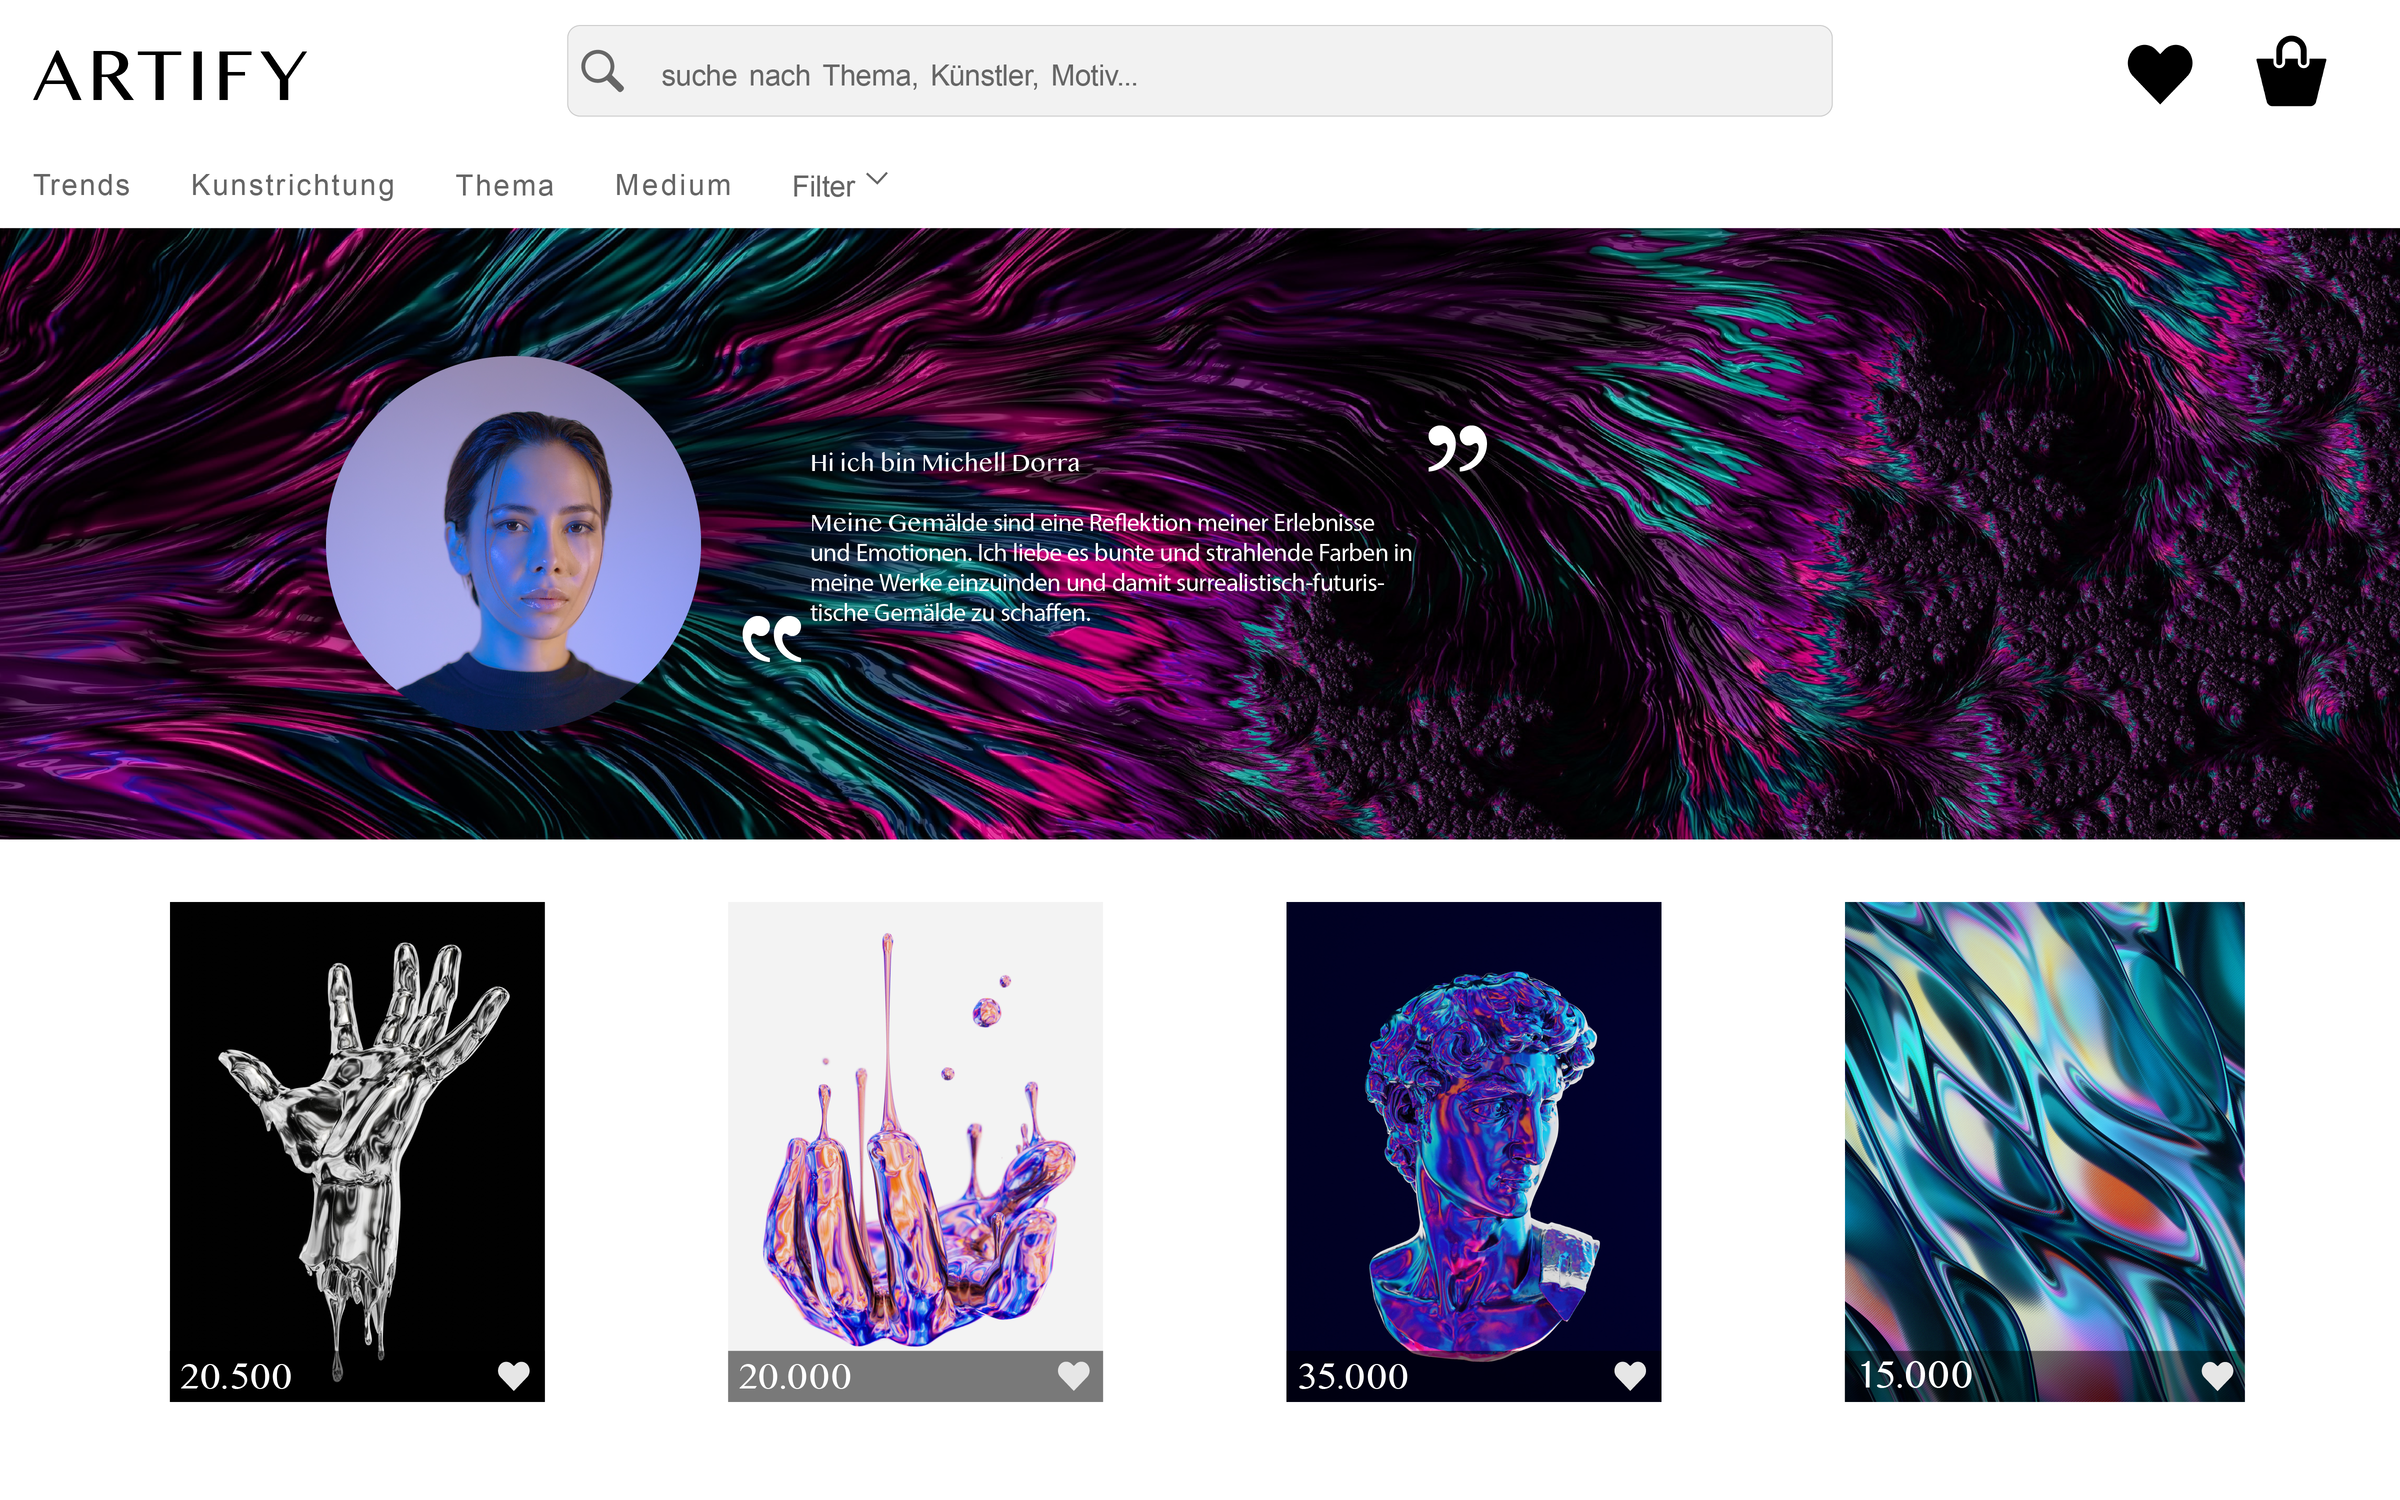
\includegraphics[width=1\textwidth]{artify-02.png}
    \caption{Individuelle Seite einer Künstlerin auf ARTIFY - Darstellung als Mockup}
    \label{3_2}
\end{figure}
%%%%%%%%%%%%%%%%%%%%%%%%%%%%%%%%%%%%%%%%%%%%%%%%%%%%%%%%%%%%%%%%%%%%%%%%%%%%%%%%%%%%%%%%%%%%%%%%%%%%%%%%%%%
\subsection{Kontext des Vorhabens}
Im Bezug auf den Kontext unseres Projektes in wirtschaftlicher und markttechnischer Sicht müssen mehrere Vektoren betrachtet werden. Auf der einen Seite existieren Plattformen wie eBay, Amazon, Etsy und Co. und auf der anderen Seite dedizierte Plattformen für den Handel mit Kunst. Diese bieten unterschiedliche Angebote und Ansätze und haben jede für sich eine eigene Zielgruppe. Der Bereich eCommerce hat sich in den leten zehn Jahren erheblich weiterentwickelt und professionalisiert. Zu beachten ist jedoch, dass die Schnittmengen von professionellem eCommerce in der Kunstbranche bisher jedoch weniger weit gefächerte Angebote bietet. \\

\begin{figure}[htb]
    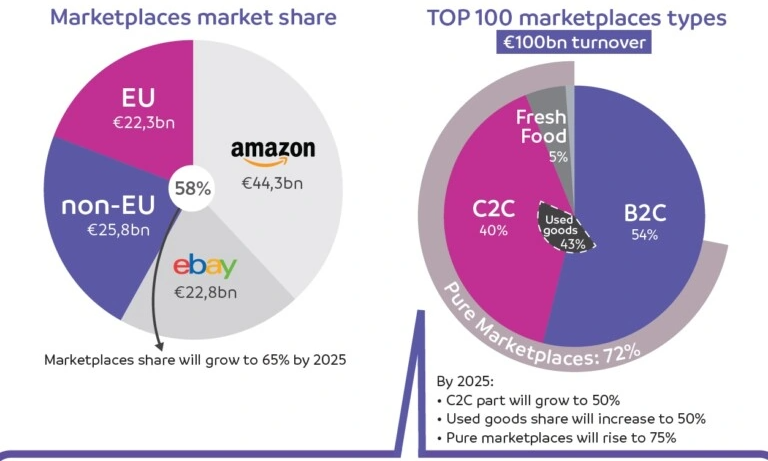
\includegraphics[width=0.8\textwidth]{contesters.png}
    \caption{Aufstellung starker Online-Vertriebsplattformen \href{https://www.e-commerce-magazin.de/online-marktplaetze-umsatz-in-cross-border-handel-steigt-auf-ueber-115-milliarden-euro/}{ (Quelle)}}
    \label{3_2}
\end{figure}

\begin{itemize}
    \item ARTIFY befindet sich im Wettbewerb mit anderen Plattformen, was den direkten Verkauf von Waren angeht.Große etablierte Player wie Amazon oder eBay sind hier marktdominierend in Sachen reinem Verkauf von Gütern und ahlungsbawicklung. Auffällig jedoch ist, dass diese Plattformen für Unikate eher eine geringe Aniehung besiten und viele potentielle Verkäuferinnen sich scheuen, ihre Kunstwerke auf Seiten zu präsentierern, auf denen sie neben DVDs und Zahnpasta verkauft werden. Diese Plattformen haben die emotionale Komponente eines Gutes aus ihren Prozessen entfernt und in diesem Punkt sehen wir uns als sehr stark und wettbewerbsfähig.
    \item Betrachtet man Anbieter wie Etsy, Redbubble und Co. so findet man dort eine wesentlich angenehmere Atmosphäre wieder, was Präsentation und Reputation der Anbieter angeht. Diese Plattformen zielen wesentlich eher auf die Produkte kleinerer Künstlerinnen und sind so prädestiniert für den Verkauf von selbsterzeugten Gütern, zudem bieten sie etwas ansprechendere Subsites für die Anbietenden. Festzustellen ist hier jedoch der Fokus auf digitale Erzeugnisse, wie den Abdruck von Postern, Kunst, Aufklebern und kleineren Erzeugnissen, wie Puppen, Basteleien und Ähnlichem. Auf diesen Plattformen wird nicht zwischen Unikaten und reproduzierbaren Produkten unterschieden, teil werden viele Produkte von Dritten gefertigt und können auf Wunsch personalisiert werden. Auch hier sehen wir eine klare Abtrennung zu unserem Anspruch an dediziertem Interesse an Unikaten und größerer Wertigkeit der Angebote.
    \item Im internationalen Wettbewerb gibt es ebenfalls Marktteilnehmer wie \glqq singulart\grqq \ die unsere Ansprüche an die Seriösität und Zielgruppe einer Plattform klar erfüllen. Diese Unternehmen haben allerdings alle internationale Sitze meist in den USA, sind teil nur auf englisch zu nutzen und würden für Support und Kommunikation die Auseinandersetzung mit unterschiedlichen rechtlichen Organisationsformen erfordern und stellen daher einen erhöhten Aufwand dar. Zudem sind diese Anbieter in Deutschland selbst in der Kunstszene nicht oder nur kaum bekannt, hier liegt der Fokus auf lokal operierenden Arteliers und anderen Anbietern.
    \end{itemize}
   
Nach genauerer Betrachtung der potentiellen Konkurrenten und der aktuellen Entwicklungen sehen wir unsere Niesche genau in dem stärker emotionalen und persönlichen Auftritt. Sowohl den schaffenden Künstlerinnen als auch den Kaufinteressenten ist es wichtig, dass Kunstwerke eine entsprechende Würdigung erfahren und entsprechend präsentiert und behandelt werden. Der Fukus ist demnach klar auf der Pärsentation der Künstlerinnen zusammen mit ihrer Kunst und nicht als Name im Hintergrund, sowie der Anspruch, dass wir nur real existierende Kunst in Form von Unikaten anbieten. Die Exklusivität jedes einzelnen Angebots ist zu betonen und es gilt zu verhindern, dass die angebotenen Werke als austauschbare Massenware erscheinen. In diesem Bereich sehen wir enormes Potential für einen Markteinstieg und mit der Positionierung in Deutschland und dem Fokus auf Kontakt und Interaktion mit den Anbietern schaffen wir ein Produkt, dass in dieser Form gerade in Deutschland noch nicht existiert.

\begin{figure}[htb]
    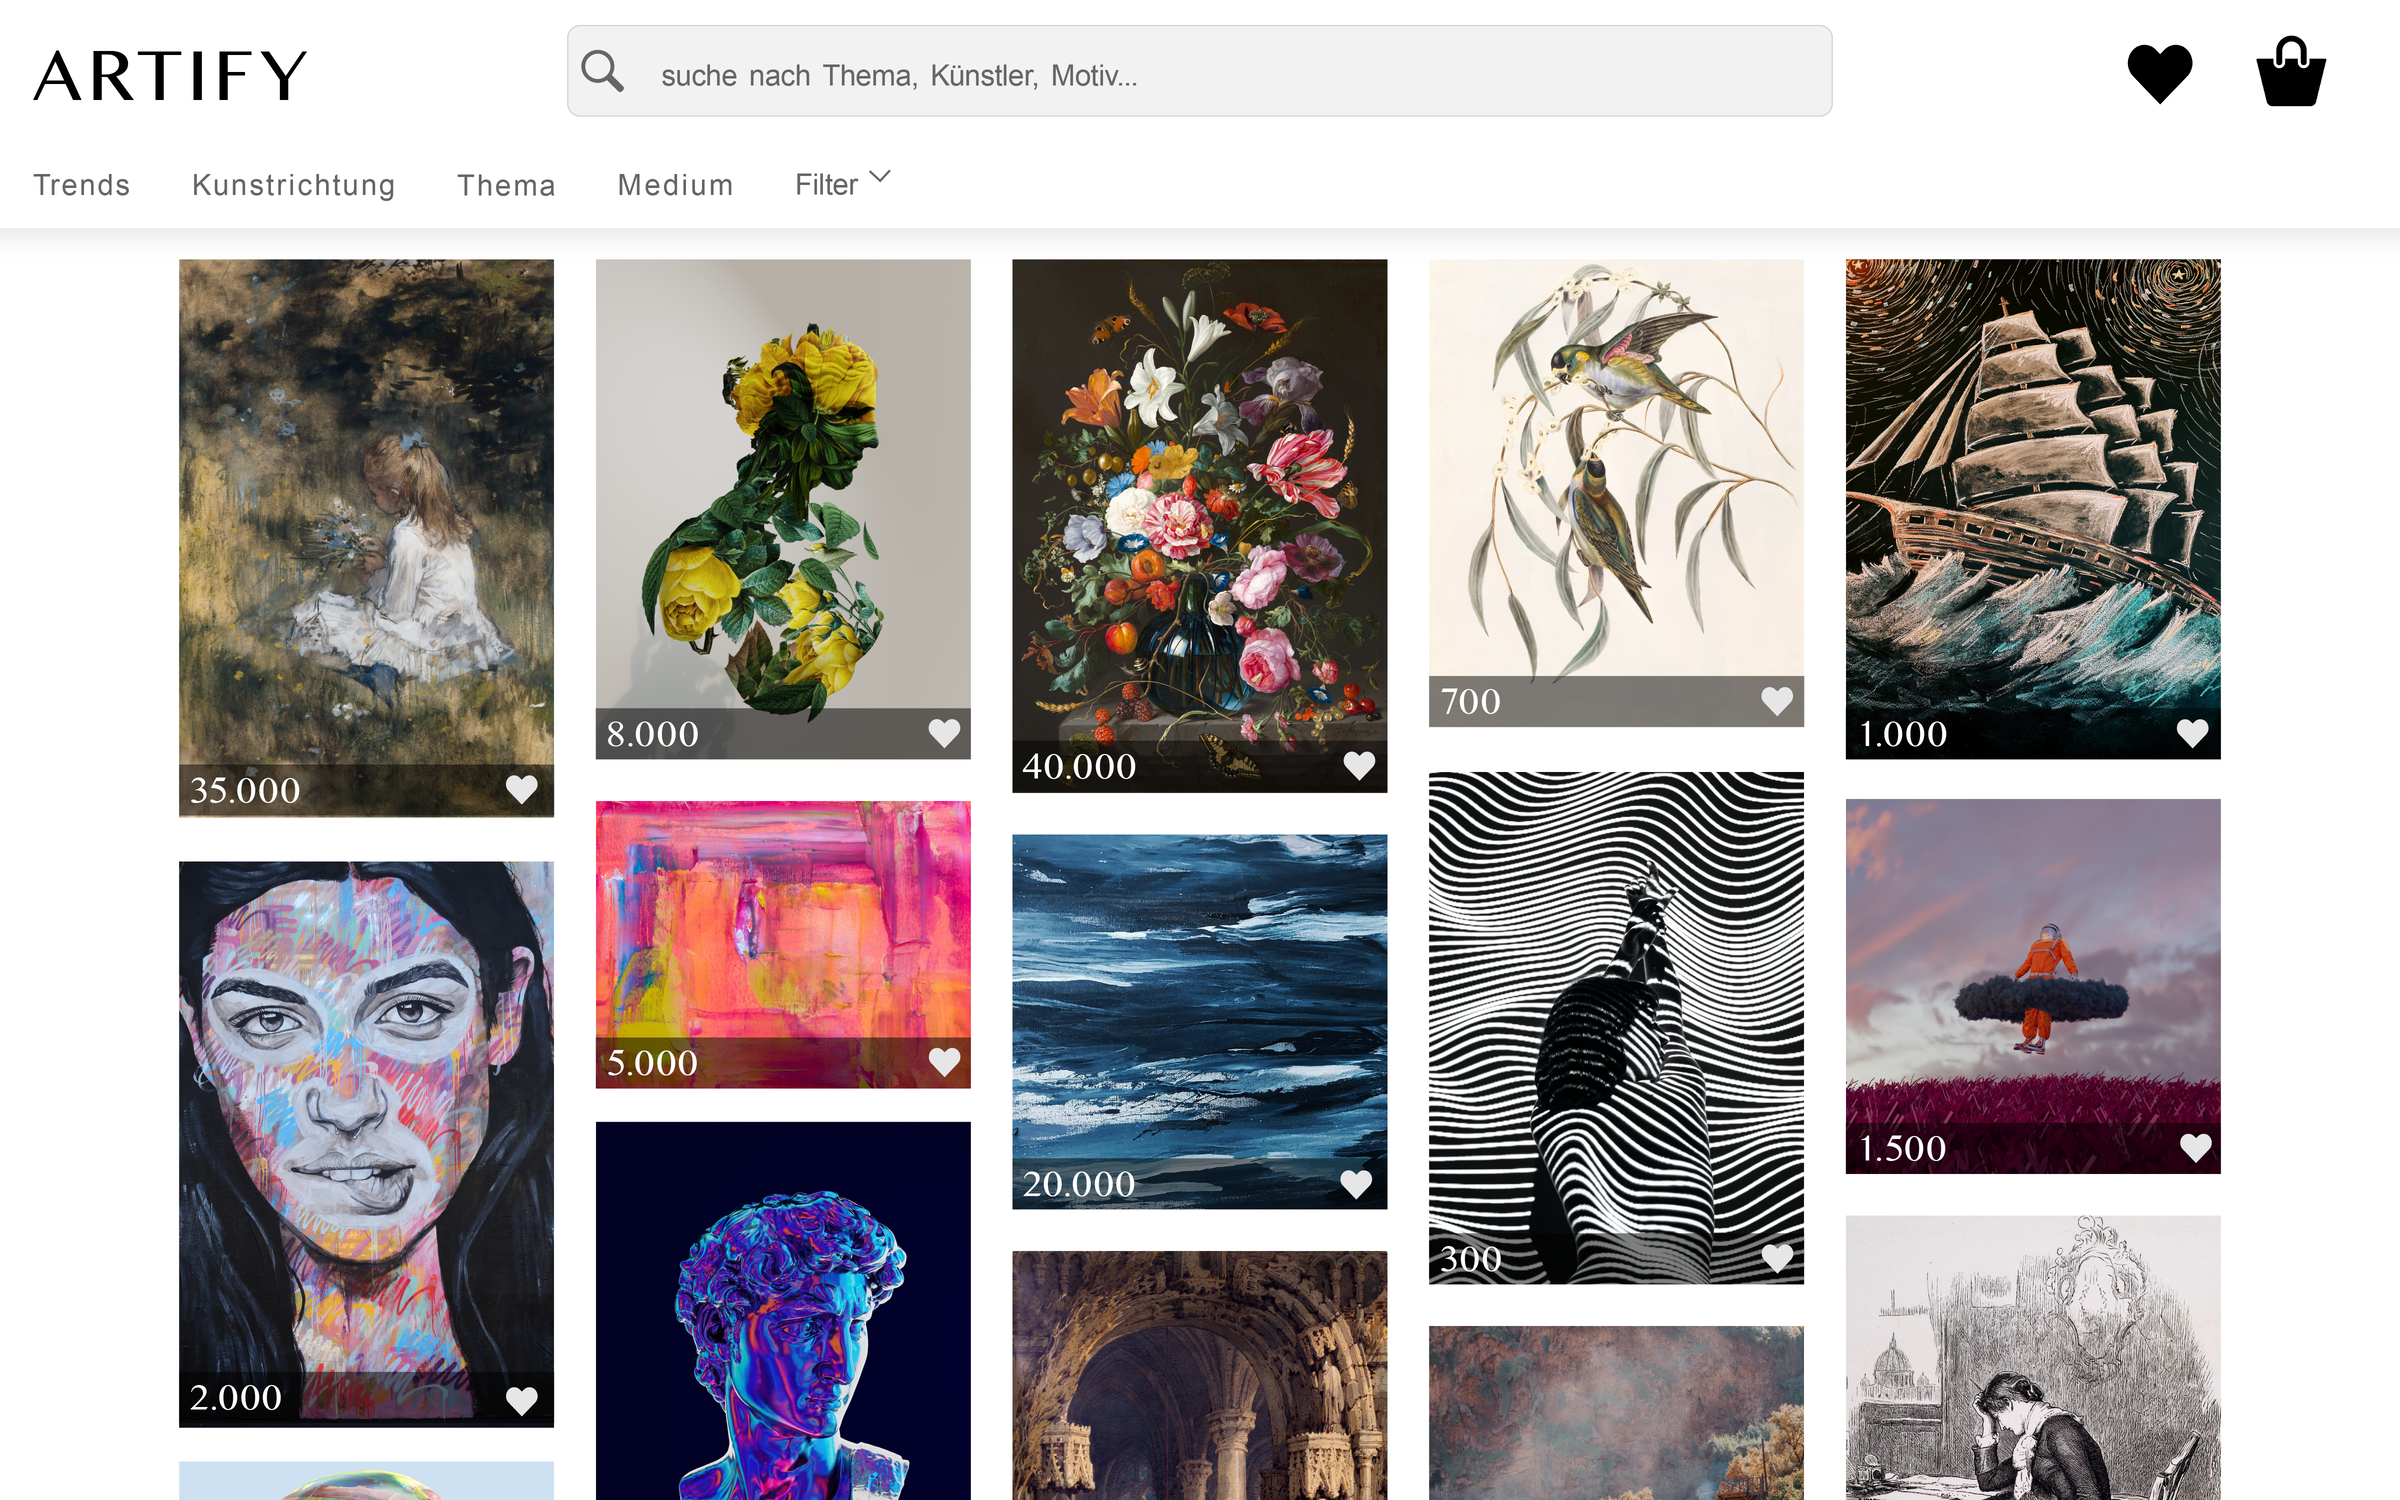
\includegraphics[width=1\textwidth]{artify-01.png}
    \caption{Landingpage von ARTIFY als Prototyp - Darstellung als Mockup}
    \label{3_2}
\end{figure}
%%%%%%%%%%%%%%%%%%%%%%%%%%%%%%%%%%%%%%%%%%%%%%%%%%%%%%%%%%%%%%%%%%%%%%%%%%%%%%%%%%%%%%%%%%%%%%%%%%%%%%%%%%%
%%%%%%%%%%%%%%%%%%%%%%%%%%%%%%%%%%%%%%%%%%%%%%%%%%%%%%%%%%%%%%%%%%%%%%%%%%%%%%%%%%%%%%%%%%%%%%%%%%%%%%%%%%%
\chapter{Das Team}
Die Mitglieder des Teams von ARTIFY bestehen aktuell aus Louisa König, Derya Aykac, Robert Kern und Jonas Rittirsch und haben sich innerhalb des Seminars Entrepreneurship an der Hochschule RheinMain kennengelernt und gemeinsam die Idee entwickelt und ausgearbeitet. Hervorzuheben ist hierbei die große Diversität der einzelnen Persönlichkeitne und ihrer individuellen Kompetenzen.
\begin{enumerate}
    \item \textbf{Louisa König} studiert Mediengestaltung und verfügt über großartrige Fachkenntnis in Feld Design und Medien und ist verantwortlich für die grafische Planung und Gestaltung der Plattform, was gerade im Kontext des Anspruchs an Seriösität und Professionalität ein großer Gewinn für das Team darstellt. Von ihr sind auch die Mockup Grafiken in diesem Dokument erstellt worden, die uns bei der Visualisierung unseres Ziel start unterstützen.
    \item \textbf{Derya Aykac} ist eine Architekturstudentin im Master und ein besonderer Gewinn für usner Team, da sie neben ihrem Studium selbst als Künstlerin tätig ist und darüber hinaus noch nütliche Kontakte in die Kunstszene mitbringt. Mit ihrer Einschätung zu Geschäftsmodell, Aufbau und Präsentation liefert sie großartiges Feedback auf der Perspektive unserer Zielgruppe der Künstlerinnen und gibt somit maßgeblich eine Richtung für zukünftige Entwicklungen und Funktionen vor.  
    \item \textbf{Robert Kern} studiert Wirtschaftsinformatik und verfügt neben technischen Knowhow auch noch über wirtschaftliches Fachwissen und Erfahrung. Durch seine bisherigen Arbeitgeber und Tätigkeiten verfügt er über Einblicke in Organisationsstrukturen von Firmen und kann sein Wissen und die Erfahrungen einbringen, um den Aufbau von ARTIFY in finanieller und struktureller Richtung voranzubringen.
    \item \textbf{Jonas Rittirsch} studiert Wirtschaftsinformatik dual und bringt neben einem starken Interesse für IT-Security Erfahrung im Bereich Organisation und Führung mit. Neben seinem Wissen in Bezug auf IT und Sicherheit, entwickelt er die Struktur des Unternehemns und seiner Prozesse anhand seiner bisherigen Erfahrungen als Projektleitung und -Organisation mit. Aufgaben im bereich Marketing und Kommunikation fallen ebenfalls in sein Gebiet. 
\end{enumerate}

Neben den festen Mitgliedern des Gründungsteams verfügen wir über Kontakte und Freunde, die uns als FullStack-Entwickler mit Knowhow im Bereich der Cross-Plattform und Appentwicklung unterstützen und damit einen wesentlichen Beitrag zun technischen Gerüst von ARTIFY beisteuern. Darüberhinaus haben sich bereits Kommilitonen gemeldet die Im Bereich Statistik und Datenanalyse ihre Fähigkeiten einbringen möchten, um uns möglichst präzises Monitoring über Wachstum, Finanzen und Reichweite zu liefern, damit wir unsere Entscheidungen daran ausrichten können. Dieses abrufbare Knowhow soll mittel- bis langfristig in die bestehende Personalstruktur integriert werden und das Wachstum des Unternehmens beschleunigen. 
%%%%%%%%%%%%%%%%%%%%%%%%%%%%%%%%%%%%%%%%%%%%%%%%%%%%%%%%%%%%%%%%%%%%%%%%%%%%%%%%%%%%%%%%%%%%%%%%%%%%%%%%%%%
%%%%%%%%%%%%%%%%%%%%%%%%%%%%%%%%%%%%%%%%%%%%%%%%%%%%%%%%%%%%%%%%%%%%%%%%%%%%%%%%%%%%%%%%%%%%%%%%%%%%%%%%%%%
\chapter{Grundlagen}
\section{Marktsituation und Ziel}
Der globale Kunstmarkt und dessen Umsätze gerade im digitalen Bereich sind enorm doch oftmals unterschätzt und übersehen. 2019 alleine wurde ein Umsatz von 60 Mrd. Euro nur duech den Verkauf von Kunstwerken erziet. Gerade hier lässt sich feststellen das Kunst im Laufe der Zeit nur äußerst selten in ihrem Wert fällt und regelmäßig weiterverkauft wird. Besonders in Zeiten wie aktuell 2020-2023 wird kunst jenseits ihres schöpferischen Aspekts auch als Wertanlage immer interessanter, gerade im Hinblick auf die Entwicklung anderer Anlageoptionen wie Immobilien, NFTs und Aktien. Ihre enorme Wertstabilität und das Wachstumspotential der einzelnen Werke bieten hier langfristig udn steigenden Zulauf an Interessenten und Käufern.\\
Für Normalverbraucher rückst diese Option erst langsam ins Bild doch das Interesse in den letzten ehn Jahren ist erheblich gestiegen und ukünftig ist kein Abbruch abzusehen. Wenn es gelingt, Neuugängen an Interessenten und Kleininvestoren hier die Hand zu reichen, lässt sich eine starke Marktposition erzielen. 
%%%%%%%%%%%%%%%%%%%%%%%%%%%%%%%%%%%%%%%%%%%%%%%%%%%%%%%%%%%%%%%%%%%%%%%%%%%%%%%%%%%%%%%%%%%%%%%%%%%%%%%%%%%
\section{Verkauf, Marketing und Standort}
\begin{enumerate}
    \item \textbf{Verkauf:} \quad Der Verkauf über und durch ARTIFY wird sich klassischen und bereits etablierten Zahlungsdienstleistern bedienen. Nach aktuellem Stand müssen Paypal, Klarna, Skrill, sowie Kredit- und Visatransaktionen abgebildet werden können. Dies bietet für uns die Möglichkeit an dieser Stelle auf bereits bekannte, etablierte und sichere Dienstleister zurückzugreifen und somit die Zahlungsabwicklung für alle Beteiligten zu vereinfachen und angenehmer zu gestalten. 
    \item \textbf{Marketing:} \quad Da es sich bei ARTIFY um eine Plattform des eCommerce handelt muss sich das Marketing zumindest in großen Teilenm der digitalen Natur des Unternehmens folgen. Als besonders effektiv wurde Werbung in den sozialen Medien festgestellt, da ein Großteil wenn nicht alle Mitglieder unserer Zielgruppe dort aktiv sind und einen wesentlichen Teil ihrer Zeit verbringen. Neben dem gedanken der Reichweite spielt dem Konzept ebenfalls in die Karten, dass der Großteil der potentiellen Künstlerinnen auf usnerer Seite bereits einen Auftriff in Social media hat, um Beispiel einen Instagram Account oder einen Pinterest-Page. Diese in große Strukturen implementierten Knotenpunkte können genutzt werden, um direkt über die Künstlerinnen als Anbieter der Werbung u arbeiten. Ein Link in der Bio oder der Caption eines Beitrags mit dem Link zu diesem Werk oder der Seite des Künstlers auf unserer Plattform wäre eine Option die Bekanntheit der Plattform zu steigern, neben konventionellen Schaltungen von zielgruppengerechter Werbung in besagten Apps und auf deren Plattformen.
    \item \textbf{Standort:} \quad Was den Standort angeht wurde bereits vermerkt, dass das RheinMain gebiet sich aus mehreren Gründen geographisch anbietet. Auf der einen Seite ist es eine strukturstarke Region mit Frankfurt, Mainz und Wiesbaden finden sich gleich drei größere Städte in einem relativ engen Ballungsraum und die Unterstützerszene in der Region um Bezug auf Startups und neue Firmen ist erstklassig. Neben den kulturellen Angeboten, Ausstellungen und Festivals der drei genannten Städte, ist Frankfurt auch eine Knotenpunkt für Verkehr und Events, einem thema mit dem sich ARTIFY zukünftig auch zunehmend beschäftigen wird, sobald die Marktetablierung abgeschlossen wurde. Da sich unser Geschäftsmodell ohne eigene Logistik oder Lagerzentren behelfen kann, spielen logistische Faktoren weniger eine Rolle als Infrastruktur und Massenerreichbarkeit.
\end{enumerate}
%%%%%%%%%%%%%%%%%%%%%%%%%%%%%%%%%%%%%%%%%%%%%%%%%%%%%%%%%%%%%%%%%%%%%%%%%%%%%%%%%%%%%%%%%%%%%%%%%%%%%%%%%%%
\section{Rechtsform}
ARTIFY wird als Gesellschaft mit beschränkter Haftung, kurz GmbH gegründet. Auf diese Weise wird die Zusammenarbeit zwischen ARTIFY und potentiellen Geldgebern und Gesellschaftern vereinfacht.
%%%%%%%%%%%%%%%%%%%%%%%%%%%%%%%%%%%%%%%%%%%%%%%%%%%%%%%%%%%%%%%%%%%%%%%%%%%%%%%%%%%%%%%%%%%%%%%%%%%%%%%%%%%
\section{Risikoanalyse}
Bei der Planung zur Unternehmensgründung von ARTIFY gibt es mehrere potentielle Risiken zu beachten. Das direkteste Risiko ist, dass nach der Gründung und dem Launch der Plattform das Interesse zur Zusammenarbeit auf Seiten der Künstlerinnen ausbleibt. Als Plattform für den Verkauf von Gütern sind wir zwingend auf die Zulieferung von außen angewiesen, da wir nicht selber produzieren. Um dem vorzubeugen sollen die ersten interessierten Künstlerinnen schon während der Entwicklungsphase aquiriert werden und direkt in den Entstehungsprozess mit eingebunden werden. So erwarten wir uns eine hohe Akeptanz und mögliche Bekanntheit schon vor dem eigentlichen Launch zu sichern.\\ 
Das zweite offensichtliche Risiko ist, dass der finanzielle Rahmen, der für die Umsetzung nötig werden würde, falsch berechnet worden ist oder sich gravierenden wirtschaftliche Zustände ändern, die uns die Ralisierung unter gegebenen Bedingungen unmöglich machen könnten. Dem können wir dank äußeren Einflüssen nicht vollständig entgegenwirken, doch wurden bei der Aufstellung der Finanzdaten Puffer an essentiellen Stellen berücksichtigt, um gegebenenfalls auftretende Unregelmäßigkeiten intern abfedern zu können. Wir sind zuversichtlich, dass wir mit unserer Kalkulation eine erfolgreiche Markteinführung realisieren können.\\
Ein weiteres Risiko wäre, dass zwar oben genannte Punkte korrekt kalkuliert und umgesetzt werden konnten, in der zweiten Finanzierungsrunde ca. ein halbes bis ein Jahr vor Erreichen des Break-Even Punktes keine Geldgeber für eine weitere Investiotionsrunde zu gewinnen sind und das Projekt so im letzten Stadium seiner Einführung scheitern könnte. Dies lässt sich vor Gründung des unternehmens nicht aus dem Weg räumen, allerdings sind wir auch hier zuversichtlich, dass wenn wir in der Lage sind zu beweisen, dass unsere bisherigen Prognosen eingetroffen sind, sich durch die Skalierbarkeit des Projekts weitere finanzielle Mittel aquirieren lassen werden.
%%%%%%%%%%%%%%%%%%%%%%%%%%%%%%%%%%%%%%%%%%%%%%%%%%%%%%%%%%%%%%%%%%%%%%%%%%%%%%%%%%%%%%%%%%%%%%%%%%%%%%%%%%%
%%%%%%%%%%%%%%%%%%%%%%%%%%%%%%%%%%%%%%%%%%%%%%%%%%%%%%%%%%%%%%%%%%%%%%%%%%%%%%%%%%%%%%%%%%%%%%%%%%%%%%%%%%%
\chapter{Realisierung}
\section{Finanzplanung}
Dieses Kapitel befasst sich mit den von uns ermittelten und aufgestellten Daten über die finanzielle Realisierbarkeit und Haushaltsplanung bezogen auf die ersten zwei Jahre nach Firmengründung mit einem besonderen Fokus auf die Break-Even Analyse und den Ausblick über das zweite Jahr hinweg. Nachfolgend finden sich alle zu beachtenden Einzelpositionen mit finanzieller Relevanz und einer Aufschlüsselung zu deren Umgang.
%%%%%%%%%%%%%%%%%%%%%%%%%%%%%%%%%%%%%%%%%%%%%%%%%%%%%%%%%%%%%%%%%%%%%%%%%%%%%%%%%%%%%%%%%%%%%%%%%%%%%%%%%%%
\subsection{Datengrundlage über zwei Jahre}
Nach Planung aller Nötigen Mittel, Dienste und Verpflichtungen errechnen wir eine Finanzaufstellung über die Ausgaben und die finanzielle Integrität des Unternehmens nach Firmengründung. Ausgegangen wird hierbei von einem Startkapitalsumme von 500T Euro.
\begin{figure}[htb]
    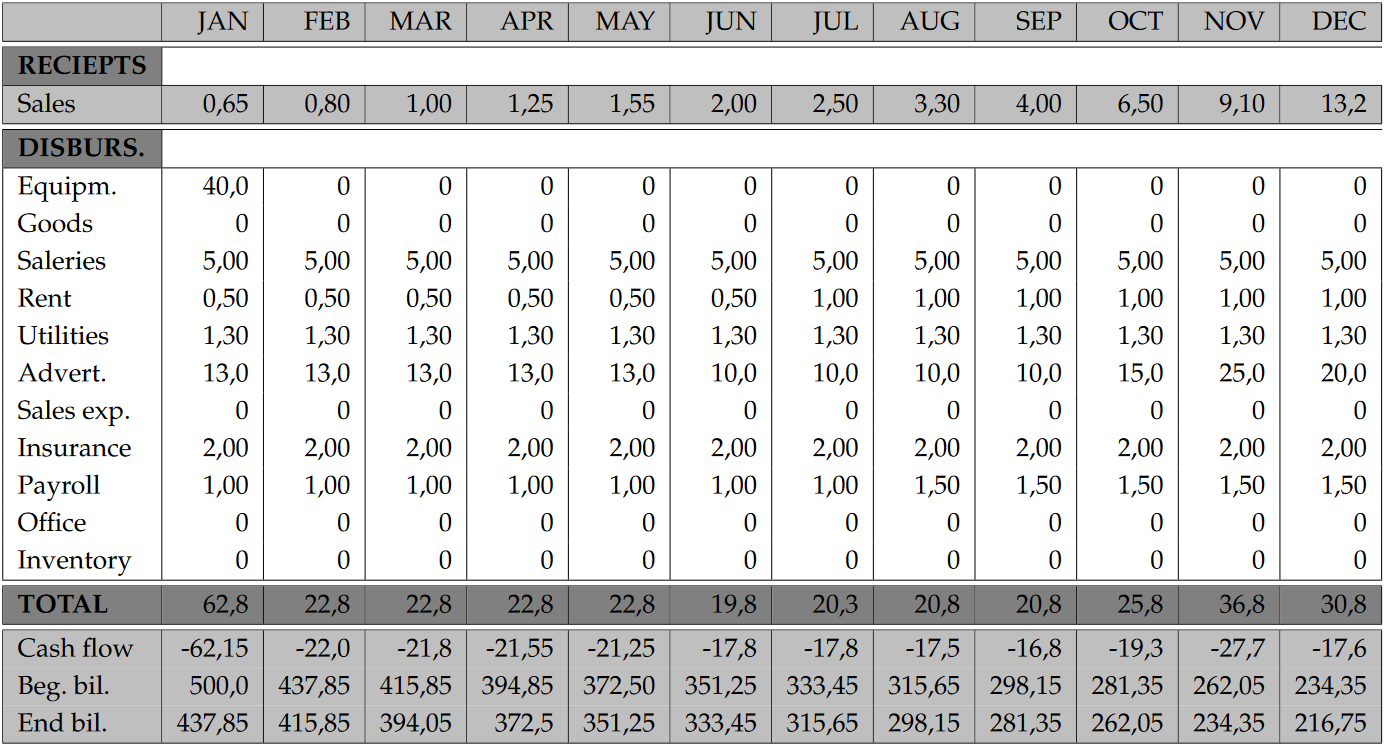
\includegraphics[width=1\textwidth]{daten1.png}
    \caption{Individuelle Aufschlüsselung der u erwartenden Kostenpositionen nach Kategorie für das erste Jahr nach Unternehmensgründung}
    \label{3_2}
\end{figure}

\begin{figure}[htb]
    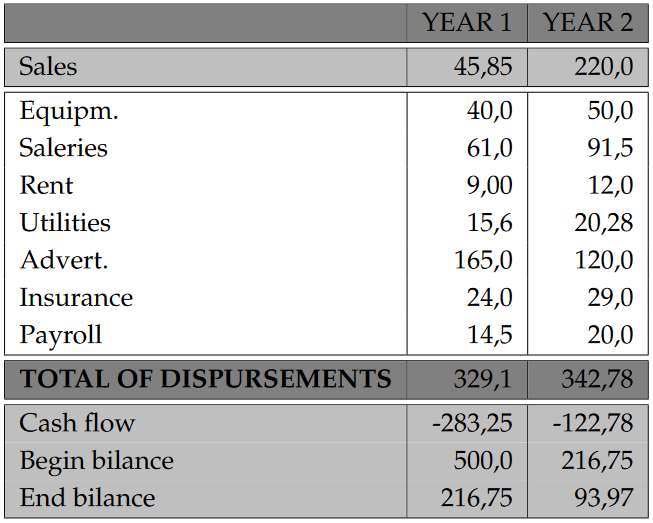
\includegraphics[width=0.6\textwidth]{daten2.png}
    \caption{Gegenüberstellung der finanziellen Hochrechnung der ersten zwei Geschäftsjahre}
    \label{3_2}
\end{figure}
\subsection{Aufschlüsselung Einzelpositionen}
\textit{Sowohl im Bereich der Einnahmen als auch der Kosten und Ausgaben werden, wie im Vorwort erwähnt, hier möglichst präzise Annäherungen versucht. Unter gegebenen Umständen können einzelne Positionen variieren. Bei der Erstellung der Datengrundlage würde jedoch darauf geachtet, dass ein gewisses Risikopuffer zur Kompensation unvorhergesehener Elemente eingeplant wird.}\\

Aus den beiden Tabellen gehen folgende Kategorien und die dazugehörigen Positionen hervor:
\begin{enumerate}
    \item \textbf{Sales:}\quad Verkäufe - hier Kommision durch abgeschlossene Transaktionen auf der Plattform. Zu beachten ist der enorm niedrige Ansatzpunkt für die ersten Monate mit einer Steigerung von 20-35\% zum Vormonat (Abhängig von Zeitpunkt im Jahr gesehen und direkte und indirekte Auswirkungen der Marketingkosten).
    \item \textbf{Equipments purchase:}\quad Hier werden nur im ersten Monat 40k € veranschlagt. Diese dienen zur Verwendung für zwei Dienstfahrzeuge, sowie deren Zulassung und für die Werbung benötigte Folierung. Hier wurde ein Puffer kalkuliert. Das Geld kann auch bei nicht vollständiger Schöpfung durch die Einkäufe für weitere zweckdienliche Objekte verwendet werden.
    \item \textbf{Cost of goods:}\quad Die reine Vermittlung und Kommissionierung von Transaktionen wirft keine direkten Kosten für das Unternehmen auf. Abnutzung durch die Verwendung von Kommunikations- und IT-Mitteln werden an späterer Stelle verbucht.
    \item \textbf{Salaries:}\quad Die veranschlagten 5000€ monatlich sehen vor, dass die bis zu vier Mitglieder des Gründerteams zwischen 1.600€ und 1250€ monatlich (quasi als Nebenverdienst auf halbe Stelle gerechnet) einziehen können. Für den November wurde ein kleines Weihnachtsgeld mit eingerechnet.
    \item \textbf{Rent:}\quad Miete im direkten Sinne fällt nicht an, da keine Verkaufs- oder Fertigungsgebäude bestehen. Die berechneten 500-1000€ monatlich sollen ggf. benötigte Konferenz- und Meetingräume abdecken, die in kooperativen Workspaces dazugebucht werden können. Die direkte Bürosituation geht von der Arbeit im Homeoffice aus. 
    \item \textbf{Utilities:}\quad Verschleiß und Ver- und Gebrauchsartikel des Teams. Fokus hierbei lieht auf elektronischer Hardware, Mobiltelefon, Internetanschluss, Zulage Energiekosten (Strom \& Heizung). Die Nutzungs- und Erneuerungskosten dieser Artikel sollen durch das Unternehmensbudget gedeckt werden.
    \item \textbf{Advertising:}\quad Einer der der, bzw. der größte Faktor der Ausgaben. Um ein Produkt wie eine Plattform zu bewerben, braucht es substantiellen Einsatz finanzieller Mittel gerade im Bereich der Netz- und social media Werbung. Geplant ist ein hoher Einstieg, der auf einen Basiswert von 10.000€ pro Monat nach dem initial burst gesenkt werden kann. Vor und in der Weihnachts- und Geschenkesaison werden dediziert mehr Kampagnen gefahren, deswegen die erhöhten Ausgaben in den Monaten November und Dezember.
    \item \textbf{Sales expenses:}\quad Transaktionen mit Zwischenhändlern, Währungstausch oder sonstiges finden nicht statt, daher eine leere Position nach aktueller Planung. Sollten Übergaben etc. weiterreichend abgesichert werden, werden hier zukünftig am Etablierung weitere Kosten entstehen.
    \item \textbf{Insurance:}\quad Gleichbleibende versicherungskosten von 2000€ in Monat für Rechtschutz und Datenschutzangelegenheiten, sowie nötige Policen bei Abwicklung über dritte Zahlungsdienstleister.
    \item \textbf{Payroll \& misc. Taxes:}\quad Unvorhergesehene Ausgaben bzgl. Positionierung von Werbung, Events und anderen Auftritten. Standgebühren, Eintritt etc.
    \item \textbf{Office expenses:}\quad Position bleibt vorerst leer, da zu Beginn keine bleibenden Büroräume und damit einhergehende Ausgaben erforderlich sind. Längerfristig werden hier gesammelte Kosten für den Unterhalt der Büroräume, Verpflegung etc. gefasst.
    \item \textbf{Inventory:}\quad Es ist mit keiner Halte- oder Vorbereitungsdauer der Objekte in unserer direkten Verantwortung zu rechnen. Sofern dies realisierbar bleibt, wird sich diese Position auch weiterhin gegen null halten lassen.
    \item \textbf{Total disbursements:}\quad Die Gesamtsumme der Ausgaben nach Monat aufgeschlüsselt. Den ersten Monat mit einer Investition von 40k € nicht mitgerechnet, pendelt diese Summe zwischen 20-30k € monatlich, je nach Saison und Werbeaufkommen.
    \item \textbf{Cash flow:}\quad Gewinn nach Abzug aller ausgehenden Beträge von der Gesamtsumme der Einnahmen durch Verkäufe/Provision. Gerade in den ersten Monaten bei einer niedrig angesetzten Startverkaufsmenge ein negativer Betrag, solange die Einnahmen gerade im ersten Jahr die Ausgaben in keiner Weise decken können.
    \item \textbf{Beginning balance:}\quad Die verbleibende Restmenge des am Monatsanfang verbleibenden Kapitals. Für diese Berechnungen wurde eine Startkapitalmenge von 500k € zugrunde gelegt. Nach allen Ausgaben startet das zweite Jahr dann mit der Restmenge von 216,75k € nach Abzügen der Kosten und Ausgaben des ersten Jahres.
    \item \textbf{Ending balance:}\quad Endstand der verfügbaren Kapitalmenge nach jedem Monat. 216,75k € nach dem ersten Jahr und 93.97k € nach dem zweiten Jahr. Die Finanzierung des Startkapitals würde nach der Berechnung für die Abwicklung der ersten zwei Jahre des Geschäfts ausreichen und mit 20\% Sicherheitsrücklage in das dritte Jahr starten.
    \end{enumerate}
%%%%%%%%%%%%%%%%%%%%%%%%%%%%%%%%%%%%%%%%%%%%%%%%%%%%%%%%%%%%%%%%%%%%%%%%%%%%%%%%%%%%%%%%%%%%%%%%%%%%%%%%%%%
\subsection{Bilanz der ersten 24 Monate}
Bei einem anteilsbasierenden Marktmodells wie dem unseren, ist es nicht verwunderlich, dass man gerade in der Anfangsphase nicht in der Lage ist, schnell schwarze Zahlen zu schreiben. Der Schlüssel zum Erfolg ist der Zugang zu den beiden Nutzergruppen der Künstler und der Kunstinteressierten. Gerade hier hängt eben der gesamte Erfolg im Verkauf an dem Aspekt des Marketing und dessen effektiven Einsatzes.\\
Berechnet an einem Startkapital von 500k € beträgt die Bilanz nach dem ersten Jahr -283,25k € bei nur 45.85k € Umsatz. Ein zu erwartend schwaches Ergebnis, bei einem frischen Markteinstieg gerade in einer derart speziellen Branche wie der Kunstszene jedoch nicht unwahrscheinlich. Im zweiten Jahr soll das forderste Ziel jedoch nicht direkt sein, mit allen Mitteln den schnellstmöglichen Break-Even Punkt zu erreichen, sondern wie in den Daten gezeigt, bei leicht reduzierten, aber dennoch weiter hohen Marketingkosten die Einnahmen zu stabilisieren. Hier rechnen wir mit einem Anstieg auf 220k €, unter der Voraussetzung, dass wir unser stetiges Wachstum von 20-30\% beibehalten können. Gerade am Anfang und nach ersten Bewährungsproben im ersten Jahr sollte dies allerdings möglich sein, weswegen wir eine weitere Investition von 50k € in das Budget aufnehmen. Diese Summe soll für marktwirksame Investitionen wie einen vergrößerten Fuhrpark, eigene Räume oder Ähnliches vorgesehen sein, bzw. als Fallschirm zur Verfügung stehen, falls einzelne Kostenpositionen spontan erheblich höher ausfallen sollten.\\
Die Ausgaben steigen somit im zweiten Jahr sogar auf 342,78€ an, dank des zu erwartenden Gewinnwachstums auf 220k € ist dieser Aufwand jedoch zu verkraften. Wenn man die zusätzliche Investition mit einberechnet und davon ausgeht, dass Positionen wie Mieten, Versicherung und andere Kosten mit dem Unternehmen mitwachsen und gegen den steigenden Gewinn gegenrechnet, dann lässt sich das zweite Jahr im Jahresabschluss also mit dem ersten vergleichen. Dies liegt aber zu einem großen Teil auch an der 50\%igen Steigerung in der Lohnzahlung, da das Modell des Nebenverdiensts zur Unternehmensgründung nun zunehmend von Aufwand und Wichtigkeit in eine volle Stelle umgewandelt werden soll. Anhand der Jahresgegenüberstellung ist zu sehen, dass dieser Schritt möglich ist und zugleich ein Polster von 20\% der ursprünglichen Gesamtsumme als Sicherheiten liquide gehalten werden kann.
%%%%%%%%%%%%%%%%%%%%%%%%%%%%%%%%%%%%%%%%%%%%%%%%%%%%%%%%%%%%%%%%%%%%%%%%%%%%%%%%%%%%%%%%%%%%%%%%%%%%%%%%%%%
\subsection{Prognose des Break-Even-Point}
Der wichtigste Punkt in der Gegenüberstellung der ersten zwei Jahre ist die Differenz des cash flow auf die beiden Jahre hochgerechnet. Während im ersten Jahr noch ein negativer cash flow von -283,25k € zu erwarten ist, wird dieser durch die steigenden Umsätze in zweiten Jahr auf -122,78k € gesenkt. Zur Erinnerung: In dieser Summe sind über 30k € für steigende Löhne und 50k € für eine größere Investition einkalkuliert. Anhand dieses Trends lässt sich sehr gut erkennen, dass sich der Break-Even Punkt des Unternehmens im dritten Jahr abzeichnet. Je nach äußeren Faktoren, ob die Investition im zweiten Jahr getätigt oder benötigt wurde, ob eine ähnliche Transaktion im dritten Jahr nötig oder abzusehen ist und wie schnell die Team-Arbeitszeit sich vollständig auf Artify konzentriert, variiert der erwartete Break-Even Punkt um einige Monate. \\
Im besten bzw. günstigsten Fall beläuft sich bei bleibendem Wachstum und keinen unvorhergesehenen Investitionsnotwendigkeiten der Punkt zwischen März und April des dritten Jahres. Selbst wenn weniger Wachstum als erwartet auftritt oder andere Kosten steigen, prognostizieren wir das Erreichen schwarzer Zahlen am dem 3. Quartal des dritten Marktjahres.
%%%%%%%%%%%%%%%%%%%%%%%%%%%%%%%%%%%%%%%%%%%%%%%%%%%%%%%%%%%%%%%%%%%%%%%%%%%%%%%%%%%%%%%%%%%%%%%%%%%%%%%%%%%
\subsection{Prognose über das dritte Jahr hinaus}
Die zweite Hälfte des dritten Jahres soll planmäßig mindestens eigenständig profitabel sein. Demnach können wir an diesem Zeitpunkt weitere Schritte zur Erweiterung und Absicherung der Unternehmung einleiten. Geplant sind hier an erster Stelle das Umstellen der Vergütung des noch vierköpfigen Teams auf branchenübliche Gehälter, sowie die Rekrutierung ein bis zwei weiterer Kräfte zur Erweiterung der Plattform, der Implementierung neuer Features und der Moderation und Kuration neuer Inhalte, Künstler und Transaktionen.\\
Ziel für das Jahr nach Break-Even ist klar das Anpassen an das Wachstum, die Verbesserung der Nutzungs- und Servicequalität, sowie das Vorstoßen in noch unbetrachtete Marktgebiete - hier die Expansion über das bisherige Nutzerfeld hinaus in den internationalen Markt, größere Kooperationen mit Werbepartnern und Partnerprogramme für Künstler, die sich Artify exklusiv als Promotion- und Vertriebsplattform vorstellen können. Der Fokus liegt hierbei klar auf der Festigung der Marke als Synonym für Qualität, Seriosität, Sicherheit und Nutzerfreundlichkeit für alle Beteiligten. Es werden feste Büroräume und eine lokale Präsenz realisiert und die Planung von ersten Events rund um die verpartnerten Künstlern soll schnellstmöglich beginnen.\\
Mittelfristig wollen wir das Ziel des Erreichen des SOM von Artify fünf Jahre nach der Gründung erreichen und die hier aufgeführten Schritte haben wir als essentiell herausgearbeitet, um als Meilensteine auf dem Weg dorthin zu dienen.
%%%%%%%%%%%%%%%%%%%%%%%%%%%%%%%%%%%%%%%%%%%%%%%%%%%%%%%%%%%%%%%%%%%%%%%%%%%%%%%%%%%%%%%%%%%%%%%%%%%%%%%%%%%
\section{Zeitplanung}
Der Zeitplan für die geplante Einführung ist der vermutlich beste Beweis für die dynamische Struktur mit der wir bis hierhin gearbeitet haben. Gerade die Anfänge sind schwer an einem Datum festzumachen, da die Entwicklung des Konzepts und des geschäftsmodels sowie unserer Prozesse schon weit vor der eigentlichen Gründungsplanung begonnen hat.\\
Um die Einführung planungskonform zu realisieren und die Zielsetzung Q4 2023 einzuhalten besteht folgender Plan:
\begin{description}
\item[03/2023] Abschluss der organisatorische Aufgaben zur Planung der Firmenstruktur. Treffen von Entscheidungen zu wesentlichen eingesetzten Produkten und Features. Beginn der Cross-Plattform Entwicklung der Anwendung.
\item[04/2023] Entwicklung des Backbone/Backend als Fundament und Flexibilität um noch einzelne Komponenten im Frontend tauschen zu können, Start Rapid Prototyping sowie erste PR Runde in der Region.
\item[05/2023] Vorstellung Prototyp im inneren Kreis beteiligter Künstlerinnen, Feedback in Entwicklungsiteration aufnehmen und Dev Log mit Updates starten.
\item[06/2023] Corporate Design, Logo, Layouts definieren, beschreiben und über Prototyp testen.
\item[07/2023] Zweite Prototyping Runde im kleinen Kreis, erneutes Feedback bzgl. UI/UX Design, Start Entwicklung im Frontend nach vorher beschlossenen Rahmenbedingungen.  
\item[08/2023] Demo Material und Prototypen nutzen und im RheinMain Gebiet auf Künstlerinnen und Arteliers zugehen und erste Nutzerstruktur etablieren.
\item[09/2023] Intensives Testing der Anwendung, Zusammenspiel aller technischen Komponenten, Port der Anwendung auf Mobilgeräte über Cross-Plattform Schnittstellen beginnen.
\item[10/2023] Finales Testen in einer geschlossenen Beta-Anwendung sowohl im Browser als auch per App. Zugang für Künstlerinnen freigeben, um erste Werke zu präsentieren. Pagebuilding der Artist-Pages und letzte Implementierung Nutzerfeedback vor Launch.
\item[11/2023] Start der Marketing-Kampagnen, Implementierung der Links zu den Werken auf den Social Media Seiten der Künstlerinnen. Entwicklung umstellen auf Monitoring und Support, Troubleshooting und Bugfixing. Launch.
\end{description}
Viele Punkte die in der Timeline spezifischen Abschnitten zugewiesen sind, haben schon im Hintergrund begonnen und werden bereits bearbeitet. Grundlegend ist die Struktur die Aufteilung in Entwicklung und Vermarktung der Plattform in einem agilen parallel laufenden System. Das direkte und frühe Feedback von Nutzern jeder Art der Plattform soll so früh und viel wie möglich Influss auf die weitere Entwicklung nehmen, um ein möglichst angenehmes Resultat zu erzeugen.\\
Parallel zu der Entwicklung wird der Fokus weiter auf der Gewinnung der ersten Nutzer für die Plattform liegen, mit dem Fokus auf Künstlerinnen, die direkt zu Launch mit ihren Werken auf der Seite starten möchten. Insgesamt ist der Zeitplan von der geschwindigkeit her gut einzuhalten, bis zum Jahresende ist ein Monat Puffer geplant der im Notfall für die Entwicklung eingesetzt werden kann. Unabhängig von Details in der Entwicklung ist die Plattform so vor Ende des Jahres und damit zur Weihnachtssaison auf dem Markt und kann mit Werbekampagnen für "das etwas andere Weihnachtsgeschenk" direkt offensiv in den Markt starten.

%%%%%%%%%%%%%%%%%%%%%%%%%%%%%%%%%%%%%%%%%%%%%%%%%%%%%%%%%%%%%%%%%%%%%%%%%%%%%%%%%%%%%%%%%%%%%%%%%%%%%%%%%%%
%%%%%%%%%%%%%%%%%%%%%%%%%%%%%%%%%%%%%%%%%%%%%%%%%%%%%%%%%%%%%%%%%%%%%%%%%%%%%%%%%%%%%%%%%%%%%%%%%%%%%%%%%%%
\chapter*{Nachwort}
\Large{Wir sagen Danke.}\\
\normalsize Im Namen des ganzen Teams aus Louisa, Dey, Robert und Jonas. Danke an alle, die uns hinter den Kulissen unterstützt und bis hierhin begleitet haben. Jenseits des Projekts für die HsRm gibt es mittlerweile Interessentinnen und Unterstützerinnen, die mit Kreativität, Kontakten, Lebenszeit und kritischen Diskussionen zuarbeiten und einen essentiellen Beitrag zum Entstehen und Fortbestehen der Unternehmung leisten. Gerade der Austausch mit Peers, Menschen aus der Szene, unseren Dozenten in diesem Seminar und unseren Freunden und Kommilitonen hat uns an einigen Stellen die Anstöße geliefert, die wir um weiterzukommen benötigt haben.\\
\\Ein besonderer Dank gilt Frau Dr. Sandra Steinbrink und dem CCC hinter ihr für das Organisieren der Veranstaltung und die Durchführung innerhalb des Semesters. Uns wurde dadurch erst das Thema der Unternehemnsgründung und die Weite des Unterstützerfeldes darin klar und ohne das Seminar wäre die Idee, das Projekt, Artify heute nicht da wo wir jetzt stehen.

\begin{comment}

\begin{figure}[htb]
    \includegraphics[width=1\textwidth]{1a}
    \caption{Anwendungsfälle als Use-Case-Diagramm}
    \label{3_2}
\end{figure}
\ \\

\begin{itemize}
    \item Startzustand
    \item Entscheidung
    \item Kreuzung
    \item Terminator
    \item Ein- und Austrittspunkt
    \item Gabelung und Vereinigung
    \item Flache Historie und Tiefe Historie
    \end{itemize}
    \cleardoublepage 

\begin{itemize}
    \item \textbf{Startzustand}:\quad Startzustände werden Sie immer 
    dann verwenden, wenn Sie den Zustand festlegen wollen, der in 
    einem Zustandsautomaten als Erstes aktiv werden soll.
    \item \textbf{Entscheidung}:\quad So wie Kreuzungen können auch 
    Entscheidungen verwendet werden, um eingehende Transitionen zu 
    einer ausgehenden Transition zusammenzufügen oder in mehrere 
    ausgehende Transitionen aufzuteilen. Die Entscheidung, welche 
    ausgehende Transition durchgeführt wird, ermitteln Guards.
    \item \textbf{Kreuzung}:\quad Sie können in Ihrem Modell 
    Kreuzungen einsetzen, wenn Sie mehrere Transitionen zu einer 
    einzigen zusammenfassen \textit{(merge)} oder eine Transition 
    auf mehrere Transitionen aufteilen möchten \textit{(split)}.
    \item \textbf{Terminator}:\quad In manchen Fällen werden Sie 
    zwischen dem „erfolgreichen“ Durchlaufen eines Zustandsautomaten 
    (per Endzustand) und einem Abbruch der Zustandsautomatenausführung 
    unterscheiden müssen. Aus diesem Grund wurde in der UML 2.0 der 
    Terminator eingeführt.

    \item \textbf{Ein- und Austrittspunkt}:\quad Um Ihnen mehrere 
    Möglichkeiten zum Betreten oder Verlassen der Zustände einer 
    solchen Hierarchie zu geben, sieht die UML 2 nun auch die 
    Verwendung von Ein- beziehungsweise Austrittspunkten vor.
    \item \textbf{Gabelung und Vereinigung}:\quad Um eine eingehende 
    Transition auf mehrere, parallel ablaufende Verhaltensbeschreibungen 
    aufzuteilen, verwenden Sie die Gabelung (im umgekehrten Fall die 
    Vereinigung).
    \item \textbf{Gabelung und Vereinigung}:\quad Der Einsatz der 
    Hierarchisierung von Zuständen und Zustandsautomaten verlangt auch, 
    sich den letzten aktiven Zustand eines Zustandsautomaten zu merken, 
    wenn während der Abarbeitung wieder zu einem bereits besuchten 
    Zustand zurückgekehrt werden soll. Dazu dient das Notationsmittel 
    der flachen und tiefen Historie.
    \end{itemize}
    \ \\
\end{comment}

% Listen wenn überhaupt ans Ende und nicht an den Anfang.
% Meist ist das aber unnötig.
% \listoffigures % Liste der Abbildungen 
%\listoftables % Liste der Tabellen
% \newpage

% \bibliographystyle{plain} % Literaturverzeichnis
% \begin{btSect}{thesis} % mit bibtopic Quellen trennen
% \section*{Literaturverzeichnis}
% \btPrintCited
% \end{btSect}
% \begin{btSect}{online}
% \section*{Online-Quellen}
% \btPrintCited
% \end{btSect}
% dann mit "bibtex thesis1" und "bibtex thesis2" arbeiten

\end{document}
;;; Local Variables:
% ;;; ispell-local-dictionary: "de_DE-neu"
;;; End:
